\documentclass[a4paper,11pt]{article}

\usepackage[latin1]{inputenc}
\usepackage[T1]{fontenc}
\usepackage[french b]{babel}

\usepackage{fancyhdr}
\usepackage{lastpage}	% pour la r\'ef\'erence \`a la derniere page (numerotation)
\usepackage{shorttoc}	% pour le sommaire

\usepackage{graphicx}

\usepackage{url}

\usepackage{lmodern}

% package geometry pour la mise en page 
\usepackage{geometry} 
\parskip 6pt %espace entre les paragraphes, tres util en mode article !
\geometry{height=24cm,width=16cm}

\usepackage{color}
\usepackage{xcolor}

\usepackage{listings}
% style de mise en page des codes sources

\definecolor{commentaires}{gray}{0.5}

\lstset{
basicstyle=\small,
keywordstyle=\bf \color{blue},
%identifierstyle=\underline,
commentstyle=\color{commentaires},
stringstyle=\color{red},
showstringspaces=false,
frameround=tttt,	% bords arrondis, t=arrondie, f=normal
frame=tblr,			% bordures
%backgroundcolor=\color{couleur_fonds_codes},
breaklines=true,
breakatwhitespace=true,
tabsize=2,
extendedchars=true,
numbers=left,
stepnumber=5,
numberstyle=\tiny,
numbersep=10pt
}
 



\title{IA41 - Delirium 2}
\author{
\textsc{Bastien CRAMILLET}
\and
\textsc{St\'ephane GENET}
\and
\textsc{Thomas KRAUSE}
\and
\textsc{Xavier MICHEL}
}
\date{\today}


% En tete et pieds de pages

\makeatletter	% pour utiliser les variables tel que le titre : \@title

\pagestyle{fancy}  	%d\'efinition du style d'en t\^ete et de pied de page
\fancyhf{}			%permet de vider les en-t\^etes et pieds de page par d\'efaut de LaTeX afin de les personnaliser
\fancyhead[C]{\it IA41 - Delirium 2}
\fancyfoot[L]{\leftmark}
\fancyfoot[R]{\thepage/\pageref{LastPage}}
\renewcommand{\footrulewidth}{2pt}		    %\'epaisseur de la ligne qui s\'epare le corps du texte et le pied de page

\makeatother


\begin{document}


\maketitle
\begin{center}
	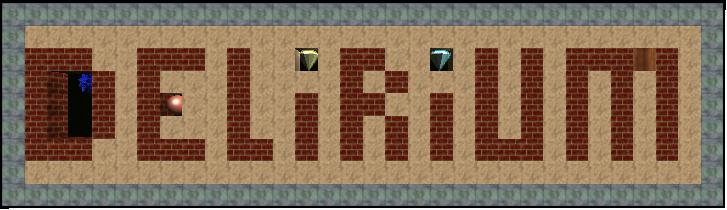
\includegraphics[width=16.5cm]{logo}
\end{center}
\thispagestyle{empty}

\newpage
\shorttableofcontents{Sommaire}{2}%
\newpage



	\section{Introduction}
	
Dans le cadre de notre UV IA41 \`a l'UTBM, nous devions r\'ealiser un projet de fin de semestre. Le choix du sujet s'est port\'e sur la cr\'eation d'une intelligence artificielle pour un jeu vid\'eo. 
Dans le cas pr\'esent, il s'agit du jeu \texttt{Delirium 2}. Dans ce jeu, le joueur dirige un mineur se d\'epla\c cant dans des galeries souterraines \`a la recherche de diamants. Sur son parcours le mineur doit \'eviter un certain nombre de pi\`eges, comme des monstres ou des rochers pouvant lui tomber sur la t\^ete. Pour chaque souterrain, le joueur doit ramasser un certain nombre de diamant sur la carte pour ensuite se rendre \`a la sortie du niveau et passer au souterrain suivant.\\

Le but du projet est donc de rendre le mineur compl\`etement autonome, ce dernier devant trouver seul son chemin pour r\'ecup\'erer les diamants, \'eviter les pi\`eges et les ennemis qui l'entourent puis rejoindre la sortie.\\

Ainsi, toutes les situations devront \^etre \'etudi\'ees pour que le mineur r\'eponde intelligemment \`a celles-ci et fasse les choix les plus judicieux pour son \'evolution.\\

Nous allons vous pr\'esenter, \`a travers ce rapport, les diff\'erents probl\`emes que peut rencontrer le mineur et pr\'esenter les solutions que nous avons impl\'ement\'ees. Mais dans un premier temps, il est n\'ecessaire de constituer une sp\'ecification d\'etaill\'ee.
	
	\newpage
	\section{Sp\'ecifications}
	
La r\'ealisation de la sp\'ecification s'est organis\'ee par l'interm\'ediaire de r\'eunions. Ces rencontres ont permis d'\'etudier les principes \'el\'ementaires requis pour une bonne \'evolution du mineur dans les souterrains. Ils nous ont permit de diviser notre travail en plusieurs parties. Chacune ayant pour r\^ole de r\'epondre \`a un probl\`eme particulier.\\

Il est \'evident que pour r\'ealiser ce projet il a fallu communiquer en dehors de ces s\'eances. Un serveur de gestion de version a  \'et\'e mis en place pour y d\'eposer notre travail et une chaine de courriels a \'et\'e utilis\'ee pour la communication sur les diff\'erents \'etats du projet.

Comme pr\'ecis\'e en introduction, le jeu D\'elirium 2 met en situation un mineur devant \'evoluer dans des souterrains et r\'epondant \`a certaines situations. Apr\`es analyse des diff\'erents niveaux d\'eja impl\'ement\'es dans le jeu de base, voici ce qui ressort de notre phase de sp\'ecifications :\\
		
		\begin{enumerate}
			\item Le mineur peut se d\'eplacer dans 4 directions primaires (vers le haut, vers le bas, vers la droite, vers la gauche)
			\item Son d\'eplacement d'une case A \`a une case B n'est possible que si la case B est de type "vide" ou "herbe"
			\item Son d\'eplacement d'une case A \`a une case B est \'egalement possible si la case B est un rocher pouvant \^etre d\'eplac\'e.
			\item Une s\'erie de rochers (allant de 1 \`a N rochers) peut \^etre d\'eplac\'ee si la case terminant la s\'erie de rochers et \'etant \`a l'oppos\'ee du mineur est de type "vide"
			\item Une s\'erie de rochers peut \^etre d\'eplac\'ee vers la droite, vers la gauche ou vers le haut si elle r\'epond aux points pr\'ec\'edents.
			\item Son d\'eplacement doit \'egalement prendre en compte des dangers pouvant provenir du haut.
			\item Un rocher peut tomber de sa position initiale si le mineur d\'eplace une s\'erie de rochers inf\'erieure, r\'ecup\`ere un diamant ou creuse une case "herbe" qui soutenait le rocher.
			\item Le mineur peut r\'ecolter un diamant en position A, en arrivant des cases situ\'ees \`a gauche, \`a droite, en haut, ou en bas de la position du diamant.
			\item Cette r\`egle peut \^etre \'eronn\'ee si le diamant est en cours de chute libre tout comme pourrait le faire un rocher (Cf : puce num\'ero 7). Dans cette situation le mineur ne peut pas r\'ecup\'erer le diamant par une case inf\'erieure sinon il meurt.
			\item Le mineur peut rencontrer des ennemis le long de son parcours.
			\item Il y a 2 types d'ennemis que nous devons prendre en compte. Les monstres bleus et monstres rouges.
			\item Ces deux ennemis doivent \^etre \'evit\'es. C'est \`a dire que le mineur ne doit pas entrer dans un p\'erim\`etre de deux cases autour du monstre.
			\item Un monstre ne peut se d\'eplacer que d'une case "vide" \`a une case "vide".
			\item Certains monstre prot\`egent des diamants. Le mineur doit dans certaines situations trouver une solution pour permettre de d\'ebloquer le diamant sans se faire attrapper par le monstre prot\'egeant le diamant.
			\item Les monstres peuvent \^etre tu\'es si un rocher leur tombe sur la t\^ete.
			\item Les souterrains peuvent contenir plusieurs types de "murs" infranchissables par les monstres et le mineur. Dans cet enssemble de murs existe des murs pouvant \^etre d\'etruits en faisant exploser un monstre \`a cot\'e un certain nombre de fois (allant de 1 fois \`a 4 fois suivant le type de mur).
			\item Certaines situations contraignent le mineur \`a devoir provoquer la destruction d'un mur pour pouvoir d\'ebloquer un passage vers une autre partie du souterrain.
			\item Une carte de souterrain est d\'efinie par un fichier XML.
			\item Afin de terminer un niveau (ou souterrain), le mineur doit r\'ecolter un nombre de diamant minimum. Ce param\`etre est d\'efinit dans le code XML de la carte.
			\item Le mineur est \'egalement contraint par un temps de jeu qu'il ne doit pas d\'epasser pour chaque niveau. Ce param\`etre est \'egalement d\'efinit dans le code XML de la carte.
			\item Le mineur doit pouvoir trouver le diamant le plus proche dans son p\'erim\`etre de vue.
			\item Le mineur doit pouvoir trouver le chemin le plus rapide d'un point A \`a un point B. En prenant en compte les \'elements cit\'es pr\'ec\'edement.
			\item Le mineur doit pouvoir abandonner un diamant qui ne sera jamais accessible. (Diamant entour\'e de murs par exemple.).
			\item Le mineur doit se concentrer sur la sortie d\`es que le nombre de diamants r\'ecolt\'es est \'egal au nombre de diamants n\'ecessaire pour terminer le niveau.
		\end{enumerate}
		
L'intelligence artificielle devra \^etre d\'evelopp\'ee gr\^ace au langage Prolog. Il sera \'egalement pr\'ef\'erable de s\'eparer les diff\'erents groupes de pr\'edicats de m\^eme famille dans des modules prolog. Nous d\'etaillerons nos modules dans la partie r\'ealisation de notre rapport.
	
	\newpage
	\section{R\'ealisation}
	
Diff\'erentes strat\'egies et algorithmes ont \'et\'e d\'evelopp\'es pour r\'epondre aux attentes de la phase de sp\'ecifications.  Qu'il s'agisse du d\'eplacement, de la recherche d'un diamant, l'\'elimination d'un ennemi ou d'un passage rendu difficile par la chute de rocher ...\\

	\subsection{Recherche du plus court chemin : Algorithme A*}
	
Une solution avait \'et\'e mise en place en d\'ebut de projet, qui consistait \`a d\'evelopper l'\texttt{Algorithme de Dijkstra}. Elle fut remplac\'ee par une m\'ethode plus adapt\'ee \`a notre probl\`eme.
		
Cet algorithme reconnu de recherche de plus court chemin dans des graphes a \'et\'e impl\'ement\'e pour g\'erer les d\'eplacements du mineur \`a partir d'un point de d\'epart donn\'e, d'un point d'arriv\'e et d'une liste repr\'esentant la carte du jeu. Il a \'et\'e impl\'ement\'e dans plusCourtChemin.pl. A partir de ces \'el\'ements l'algorithme \'etudie les directions possibles que peut prendre le mineur. Consid\'erons la carte de jeu comme un tableau, chaque direction possible ajoute un lien entre la case o\`u se trouve le mineur et celle o\`u il peut aller, d\'efinissant ainsi un chemin possible. Tous les chemins possibles sont retenus dans une liste dite \textit{"ouverte"}, les chemins que le mineur ne peut pas prendre, comme par exemple un mur ou un rocher bloquant le passage, sont retenus dans une liste dite \textit{"ferm\'ee"}.  L'op\'eration de recherche d'une direction possible est r\'ep\'et\'ee \`a partir des chemins contenus dans la liste ouverte jusqu'\`a atteindre le point d'arriv\'ee. Si un chemin s'av\`ere \^etre inefficace et n'abouti \`a rien, il sera \`a son tour ins\'er\'e dans la liste ferm\'ee et retir\'e de la liste ouverte. Le chemin semblant \^etre le plus court sera prioritaire et le mineur l'empruntera.

\begin{center}
\texttt{Compl\'ement d'informations \`a cette adresse : \url{http://fr.wikipedia.org/wiki/Algorithme_A*}}
\end{center}

	\subsection{Strat\'egie de recherche du plus proche diamant}
	
		\subsubsection{Situation simple}
		
Dans le cas le plus simple, le mineur va chercher \`a aller au diamant le plus proche de lui. Par exemple sur la figure ci-dessous, le mineur va tracer son chemin vers le diamant num\'ero 1 puis se d\'eplacer. Apr\`es ce d\'eplacement il recherchera le dimant qui sera le plus proche de lui (\`a nouveau le 1) ; il se d\'eplacera donc \`a nouveau dans la direction de ce diamant, et ainsi de suite\dots

		\begin{figure}[h]
			\center
			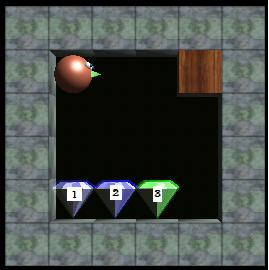
\includegraphics[width=5cm]{simple1}
			\caption{\label{simpleRechercheDiamant} Repr\'esentation d'une situation simple de recherche du plus proche diamant}
		\end{figure}
		
		\subsubsection{Situation plus complexe}
		
En r\'ealit\'e, il arrive tr\`es souvent que le diamant le plus proche du mineur soit inaccessible auquel cas on va pr\'ef\'erer s'int\'eresser au diamant suivant. Par exemple sur la figure suivante, le diamant 1 est inaccessible, le mineur va alors rechercher au diamant num\'ero 2. Ce dernier \'etant \'egalement inaccessible, le mineur va alors se d\'eplacer vers le diamant not\'e 3.
	
		\begin{figure}[h]
			\center
			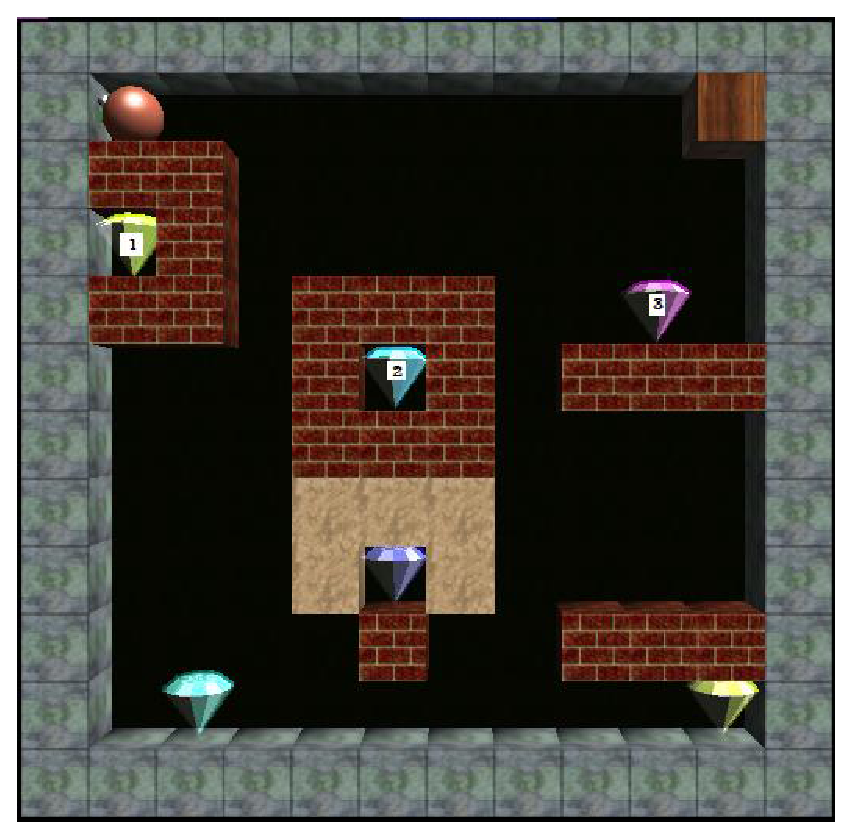
\includegraphics[width=9cm]{simple2}
			\caption{\label{complexeRechercheDiamant} Repr\'esentation d'une situation complexe de recherche du plus proche diamant}
		\end{figure}
		
	\newpage
	\subsection{D\'eplacement de rochers}
	
La strat\'egie de d\'eplacement de rochers est tr\`es simple.\\
Tout d'abord il faut savoir que le mineur \'evite le plus possible de d\'eplacer des rochers. S'il peut effectuer le d\'eplacement sans d\'eplacer de rochers, il le fera. Cette technique permet au mineur de ne pas bloquer stupidement ses objectifs. Par exemple sur la situation ci-dessous le mineur est tent\'e de partir sur la gauche \`a son premier d\'eplacement auquel cas il bloquera la sortie. Gr\^ace \`a l'utilisation du chemin sans d\'eplacement de rochers, la sortie reste disponible.

		\begin{figure}[h]
			\center
			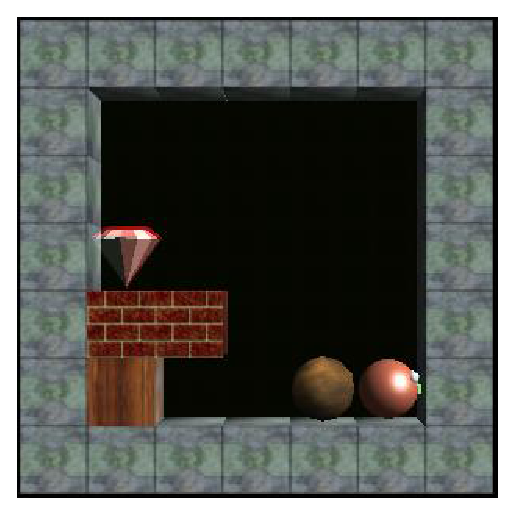
\includegraphics[width=5cm]{rochers1}
			\caption{\label{deplacementRocher1} Situation o\`u le d\'eplacement d'un rocher est possible mais pas n\'ec\'essaire}
		\end{figure}
		
Cependant le mineur est apte \`a d\'eplacer les rochers ci cela devenait n\'ecessaire, sur une profondeur choisit arbitrairement qui est de 5 rochers. Par exemple il peut pousser 5 rochers sur sa gauche si la situation s'y pr\^ete (pas d'obstacle derri\`ere les rochers\dots). Par exemple dans la situation ci-dessous le mineur va bien \'evidemment d\'eplacer les rochers pour se sortir de cette situation.

		\begin{figure}[h]
			\center
			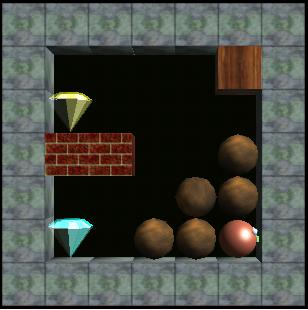
\includegraphics[width=5cm]{rochers2}
			\caption{\label{deplacementRocher2} Situation o\`u le d\'eplacement d'un rocher est obligatoire}
		\end{figure}
		
\newpage
Les rochers se d\'eplacent parfois seuls, comme dans le cas d'une chute sur le mineur. Dans ce cas le mineur va alors d\'etecter qu'il est menac\'e et il esquivera les rochers tombant en se d\'ecalant sur la gauche ou sur la droite selon les possibilit\'es et l'objectif \`a atteindre.

		\begin{figure}[h]
			\center
			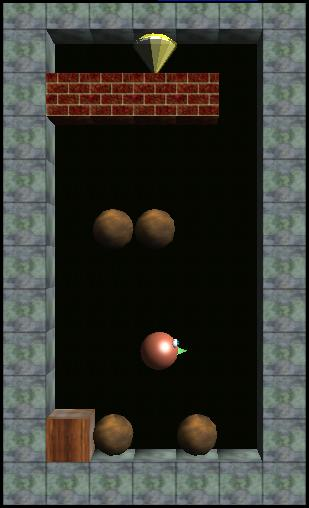
\includegraphics[width=5cm]{rochers3}
			\caption{\label{deplacementRocher3} Chute libre de plusieurs rochers sur le mineur}
		\end{figure}
		\clearpage
		
	\newpage
	\subsection{Strat\'egie mise en place pour \'eviter un monstre}
	
		\subsubsection{Cas g\'en\'eral}
		
		Pour le cas g\'en\'eral, d\`es que le mineur rencontre un monstre dans son champ de vision, la liste repr\'esentant le tableau de cases visibles par le mineur est modifi\'ee avant de lui laisser chercher le plus court chemin vers le prochain diamant ou la sortie.\\
Chaque monstre pr\'esent dans le champ de vision du mineur est alors encercl\'e de murs \`a 2 cases aux alentours. L'algorithme A* recherchera donc un chemin lui permettant d'\'eviter le monstre. Bien entendu les murs ajout\'es pour \'eviter le monstre ne sont pas visible pour le joueur.

		\begin{figure}[h]
			\center
			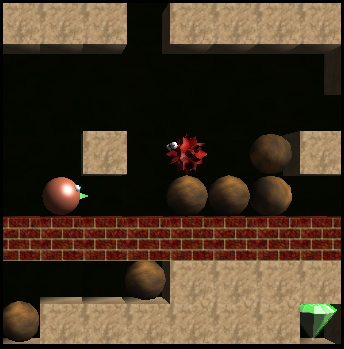
\includegraphics[width=5cm]{monstre1}
			\caption{\label{monstre1} Monstre mettant en danger le mineur : vision du joueur}
		\end{figure}
		
		\begin{figure}[h]
			\center
			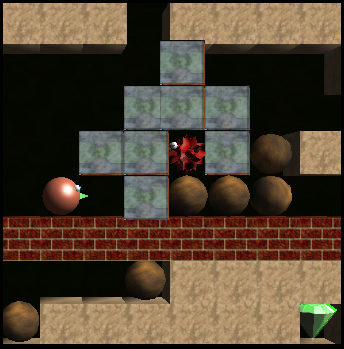
\includegraphics[width=5cm]{monstre2}
			\caption{\label{monstre2} Monstre mettant en danger le mineur : vision technique }
		\end{figure}
		
		\subsubsection{Cas plus complexe}
		
Afin de ne pas perturber l'environnement de la carte. Seules les cases accessibles par le mineur (case vide et case d'herbe) sont remplac\'ees par des murs.
Mais nous aurions \'egalement pu avoir cette configuration :
	
		\begin{figure}[h]
			\center
			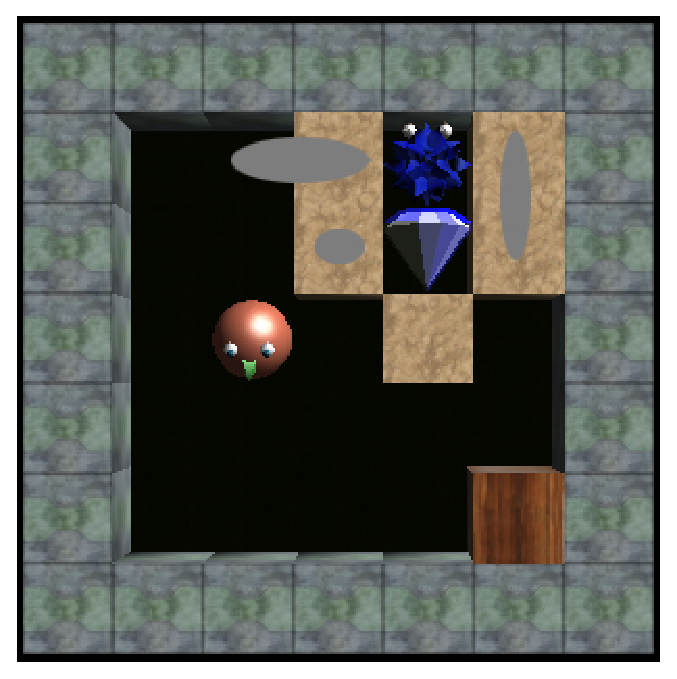
\includegraphics[width=5cm]{situation1}
			\caption{\label{monstre3} Limite de la construction de murs autour d'un monstre }
		\end{figure}
		
Sur cette repr\'esentation seules les cases marqu\'ees d'un marqueur gris seront remplac\'ees par des murs. Le diamant n'est pas remplac\'e, ni la case herbe du dessous. Nous ne remplaçons donc pas la case de niveau sup\'erieur \`a une case non remplac\'ee. Ici la case herbe est au niveau 2 du champ de vision du monstre, le diamant au niveau 1 est bloquant pour la case herbe. La case herbe n'est donc pas remplac\'ee.
Cette repr\'esentation nous permet de r\'esoudre certaines situations.
	
	\newpage
	\subsection{Situation particuli\`ere 1 : Dimant pi\'eg\'e par un monstre}
	
		\subsubsection{Aper\c cu de la situation}
		
		Sur certaines cartes, un monstre peut bloquer l'acc\`es au mineur \`a un diamant. Voici un aper\c cu de la situation :
		
		\begin{figure}[h]
			\center
			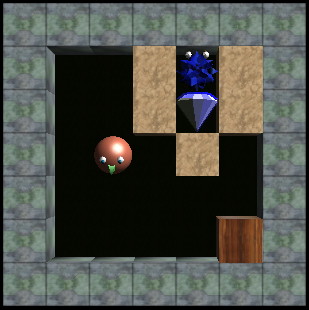
\includegraphics[width=5cm]{situation12}
			\caption{\label{situation1} Aper\c cu de la situation particuli\`ere 1 }
		\end{figure}
			
		\subsubsection{R\'esolution de la situation}
		
Afin de r\'esoudre cette situation, le mineur devra creuser la case herbe situ\'ee en dessous du diamant, puis s'\'ecarter pour laisser tomber le diamant. L'algorithme standard de recherche du plus proche diamant et l'encerclement du monstre par des murs permettra ensuite au mineur de r\'esoudre cette carte. Voici une image explicative de la solution :

		\begin{figure}[h]
			\center
			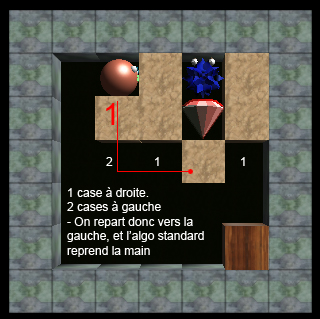
\includegraphics[width=5cm]{situation111}
			\caption{\label{situation1reso} R\'esolution de la situation particuli\`ere 1 }
		\end{figure}
	
	\newpage
	\subsection{Situation particuli\`ere 2 : Attaque des montres}
	
	Cette strat\'egie est impl\'ement\'ee dans situation2.pl. Elle consiste \`a neutraliser un ennemis dans une situation donn\'ee que nous allons d\'etailler par la suite. Elle se d\'ecompose en trois phases.

	\subsubsection{Phase 1 : rep\'erer la situation}
	
La situation doit se pr\'esenter sous la forme suivante : un monstre se prom\`ene sur une ligne bloqu\'ee sur une courte distance. Au dessus de cette ligne se trouve une ligne d'herbe. Enfin, un rocher doit \^etre pr\'esent au dessus de la ligne d'herbe en bout de course du monstre. La situation typique est r\'esum\'ee sur l'image ci-dessous.  
	
		\begin{figure}[h]
			\center
			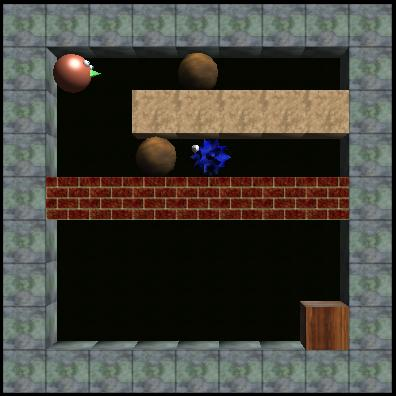
\includegraphics[width=5cm]{situation2-1}
			\caption{\label{situation21} Phase 1 de r\'esolution de la situation 2 }
		\end{figure}
	
Cette situation \'etant rep\'er\'e, le mineur va alors se mettre en position en s\'ecurit\'e comme sur l'image ci-dessous.
	 
		\begin{figure}[h]
			\center
			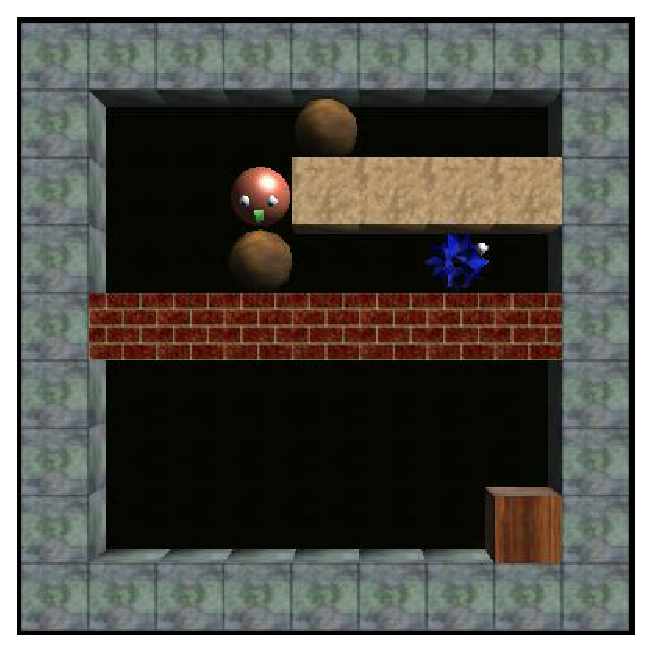
\includegraphics[width=5cm]{situation2-2}
			\caption{\label{situation22} Phase 1 de r\'esolution de la situation 2 }
		\end{figure}
	 
	 \newpage
	\subsubsection{Phase 2 : placement sous le rocher}
	
Le mineur est \`a ce moment en position d'attente, il va alors attendre que le monstre se situe \`a quatre cases de distance \`a partir de sa but\'ee \`a gauche pour se placer sous le rocher et se mettre en position d'attente, comme mis en image ci-dessous.

	\begin{figure}[h]
			\center
			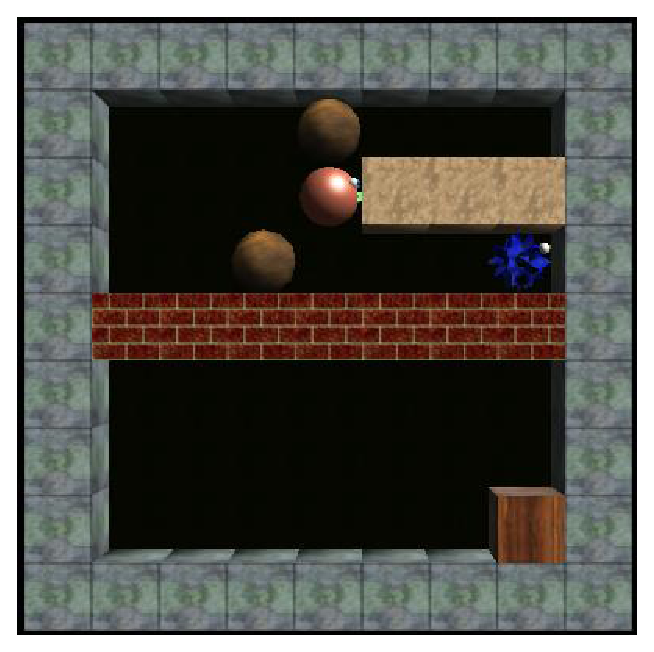
\includegraphics[width=5cm]{situation2-3}
			\caption{\label{situation22} Phase 2 de r\'esolution de la situation 2 }
		\end{figure}
		
	\subsubsection{Phase 3 : D\'eclenchement du pi\`ege}
	
Enfin, lorsque le monstre s'approche, le mineur va s'\'ecarter de sous le rocher de façon \`a ce que celui-ci tombe sur le monstre. Ainsi le monstre est neutralis\'e.

		\begin{figure}[h]
			\center
			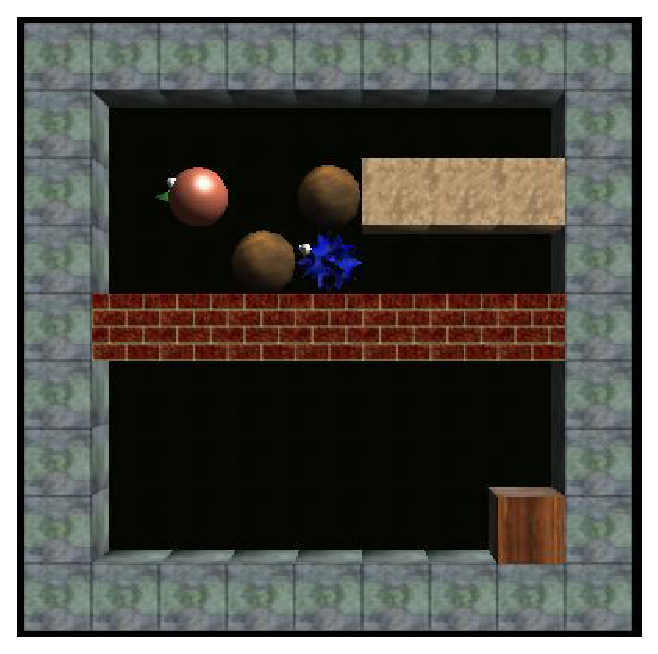
\includegraphics[width=5cm]{situation2-4}
			\caption{\label{situation22} Phase 3 de r\'esolution de la situation 2 }
		\end{figure}
		
	\newpage
	\subsection{EXTRA : Editeur de carte Html/JavaScript}
	
D\`es le d\'ebut du projet, il nous \'etait difficile de concevoir des cartes r\'esumant une situation particuli\`ere. Nous n'arrivions pas \`a visualiser correctement ce que nous concevions comme carte dans le fichier XML. Nous avons donc pens\'e \`a concevoir un \'editeur de carte Delirium 2.0 en HTML \/ JavaScript.

	\begin{figure}[h]
			\center
			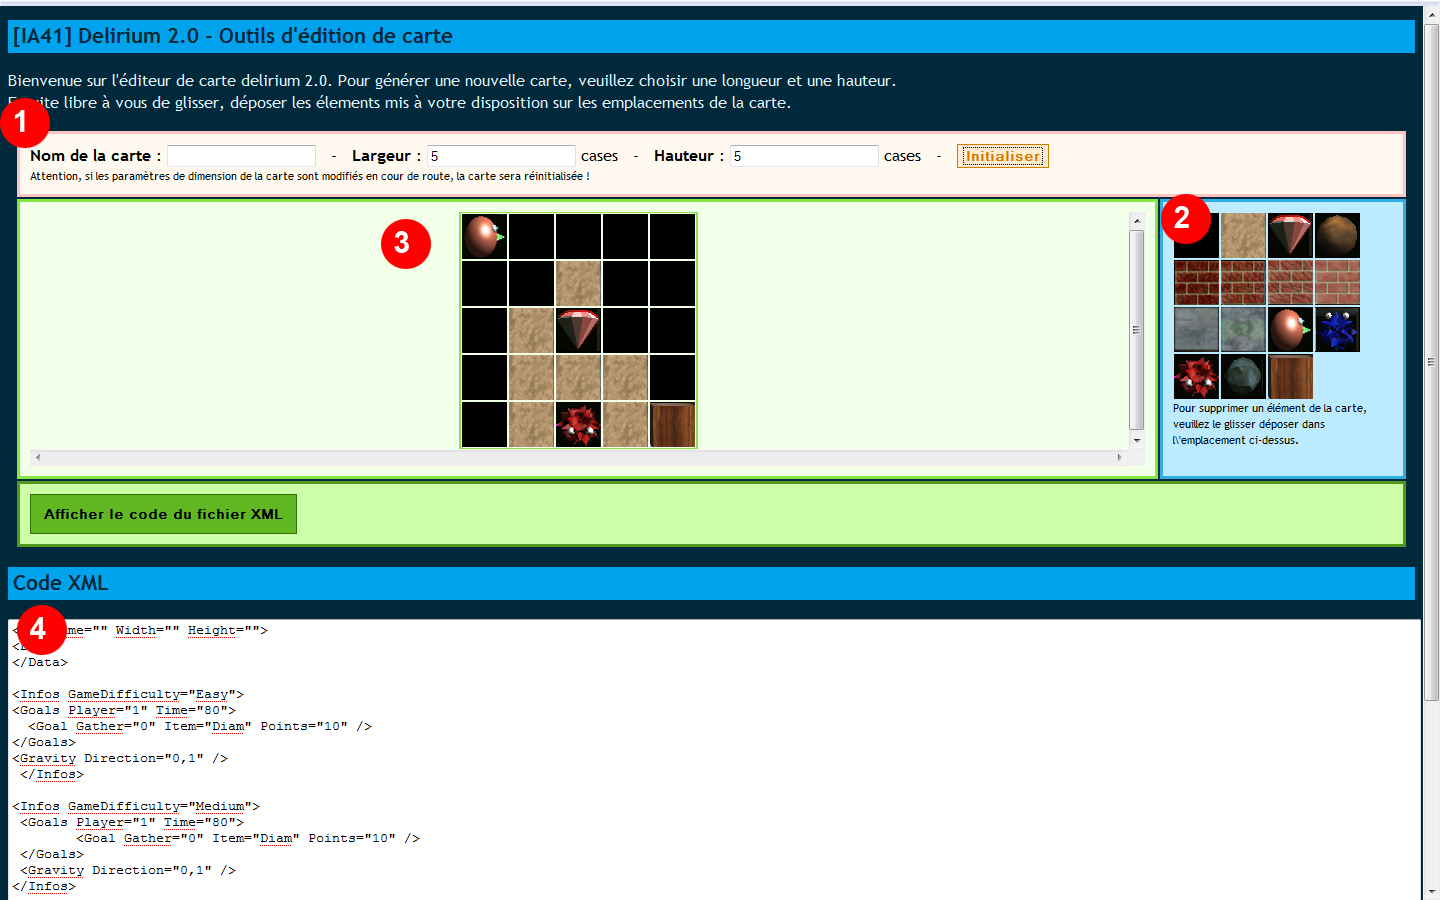
\includegraphics[width=12cm]{editeur}
			\caption{\label{situation22} Editeur de carte Delirium 2 }
		\end{figure}
		
	\begin{enumerate}
		\item Nous renseignons les informations de la carte
		\item Nous avons \`a disposition les \'el\'ements de la carte
		\item Nous pouvons glisser depuis le \og{} 2 \fg{} les \'el\'ements de la carte sur la carte.
		\item Le code XML du fichier est g\'en\'er\'e automatiquement.
	\end{enumerate}
	
	\newpage
	\section{Conclusion}
	
Lors de ce projet de plusieurs mois, nous devions r\'ealiser l'intelligence artificielle du h\'ero d'un jeu vid\'eo, le permettant de se d\'eplacer, de r\'ecup\'erer ses objectifs de mission, \`a savoir, des diamants, ainsi qu'\'eviter les ennemis qui le pourchassent et les pi\`eges tendus par le d\'ecor et ses rochers. Aujourd'hui, notre h\'ero est tout \`a fait capable de se d\'ebrouiller dans ce genre d'environnement, en prenant la direction des diamants et en \'evitant ou \'eliminant les ennemis, se servant m\^eme de l'environnement pour s'en sortir indemne. Les objectifs que nous nous \'etions pos\'es ont donc \'et\'e remplis.\\

De nombreuses difficult\'es ont \'et\'e rencontr\'ees, comme pour l'impl\'ementation de l'algorithme A* qui est quelque peu d\'elicat \`a programmer ou les situations d'esquive et d'\'elimination des ennemis. Travailler avec un langage r\'ecursif n'est pas non plus chose ais\'e au d\'ebut.

Le travail que nous avons r\'ealis\'e peut tout \`a faire \^etre am\'elior\'e, notamment au niveau de la rapidit\'e d'ex\'ecution qui est parfois assez lente, principalement lors de passages complexes ou de nombreux chemins sont possibles pour notre h\'ero.  
	


\newpage
\section{Codes sources du programme}

\subsection{ai-00.pl}
\lstinputlisting[language=prolog]{ai-00.pl}

\newpage
\subsection{eviterMonstre.pl}
\lstinputlisting[language=prolog]{eviterMonstre.pl}

\newpage
\subsection{outilsCarte.pl}
\lstinputlisting[language=prolog]{outilsCarte.pl}

\newpage
\subsection{plusCourtChemin.pl}
\lstinputlisting[language=prolog]{plusCourtChemin.pl}

\newpage
\subsection{rochers.pl}
\lstinputlisting[language=prolog]{rochers.pl}

\newpage
\subsection{situations.pl}
\lstinputlisting[language=prolog]{situations.pl}

\newpage
\subsection{situations2.pl}
\lstinputlisting[language=prolog]{situations2.pl}

\newpage
\tableofcontents

\end{document}

